%!TEX root = Manuscript.tex

\chapter{Comparison between $SuperGlue_{tiling}$ and $SuperGlue_{orig}$}
\label{chap:appendix2}
In order to explore whether the \textit{one-to-many tiling scheme} improves the performance of SuperGlue, we compare the results of SuperGlue with and without the \textit{one-to-many tiling scheme} (i.e. $SuperGlue_{tiling}$ and $SuperGlue_{orig}$) on matching orthophotos and DSMs. We chose the orhtophotos and DSMs from Fr{\'e}jus 1970 and 2014 individually for testing.\\
\section{Comparison on matching orthophotos}
Figure~\ref{MatchOrtho} displayed the results of matching orthophotos with $SuperGlue_{tiling}$ and $SuperGlue_{orig}$. As can be seen, the former recovered 58 good matches with an inlier ratio of 33\%, while the latter failed to find any correct matches.\\
\begin{figure*}[htbp]
	\begin{center}
		\subfigure[Orthophotos]{
			\begin{minipage}[t]{0.48\linewidth}
				\centering
				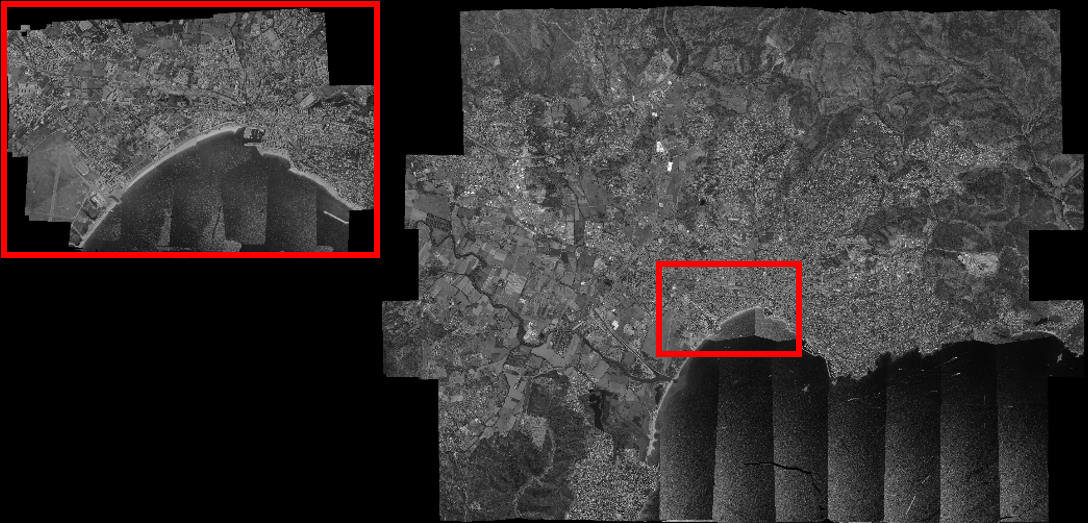
\includegraphics[width=7.5cm]{images/Chapitre3/Ortho-MEC-Malt_Tapas_1970_Ortho-MEC-Malt_2014.png}
			\end{minipage}%
		}
		\subfigure[Number of recovered matches]{
			\begin{minipage}[t]{0.48\linewidth}
				\centering
				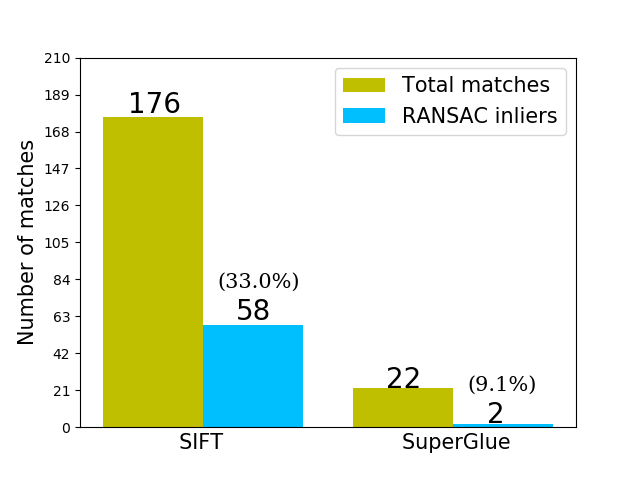
\includegraphics[width=4.8cm]{images/appendix2/PlotCurves_TileTest-Ortho-MEC-Malt_Tapas_1970_Ortho-MEC-Malt_2014.png}
			\end{minipage}%
		}
		\subfigure[$SuperGlue_{ours}^{RANSAC Inliers}$]{
			\begin{minipage}[t]{0.48\linewidth}
				\centering
				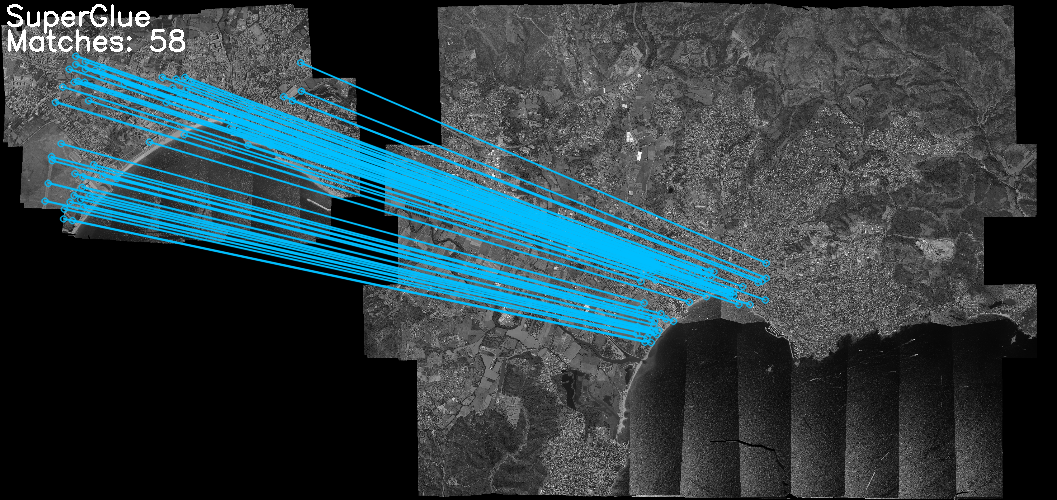
\includegraphics[width=6cm]{images/Chapitre3/Homol-SubPatch_R270-2DRANSAC_Ortho-MEC-Malt_Tapas_1970_Ortho-MEC-Malt_2014.png}
			\end{minipage}%
		}
		\subfigure[$SuperGlue_{orig}^{TotalMatches}$]{
			\begin{minipage}[t]{0.48\linewidth}
				\centering
				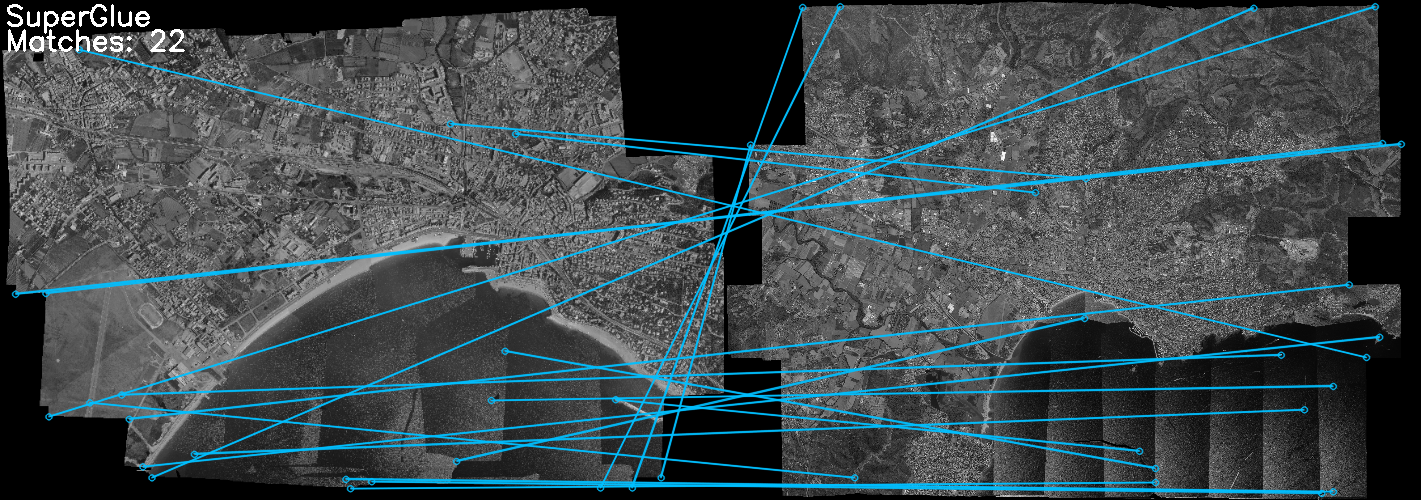
\includegraphics[width=6cm]{images/appendix2/Homol-SuperGlue_Ortho-MEC-Malt_Tapas_1970_Ortho-MEC-Malt_2014.png}
			\end{minipage}%
		}
		\caption{Comparison between $SuperGlue_{tiling}$ and $SuperGlue_{orig}$ on orthophotos from Fr{\'e}jus 1970 and 2014 individually. (a) Orthophotos to be matched, with red rectangles indicating the common zone. (b) Numbers of total matches, GT inliers and RANSAC inliers of $SuperGlue_{tiling}$ and $SuperGlue_{orig}$. (c) Visualization of RANSAC inliers based on $SuperGlue_{tiling}$. (d)Visualization of total matches based on $SuperGlue_{orig}$.}
		\label{MatchOrtho}
	\end{center}
\end{figure*} 

\section{Comparison on matching DSMs}
Figure~\ref{MatchDSM} displayed the results of matching DSMs with $SuperGlue_{tiling}$ and $SuperGlue_{orig}$. As can be seen, the former recovered 190 good matches with an inlier ratio of 46.5\%, while the latter failed to find any correct matches.\\
\begin{figure*}[htbp]
	\begin{center}
		\subfigure[DSMs]{
			\begin{minipage}[t]{0.48\linewidth}
				\centering
				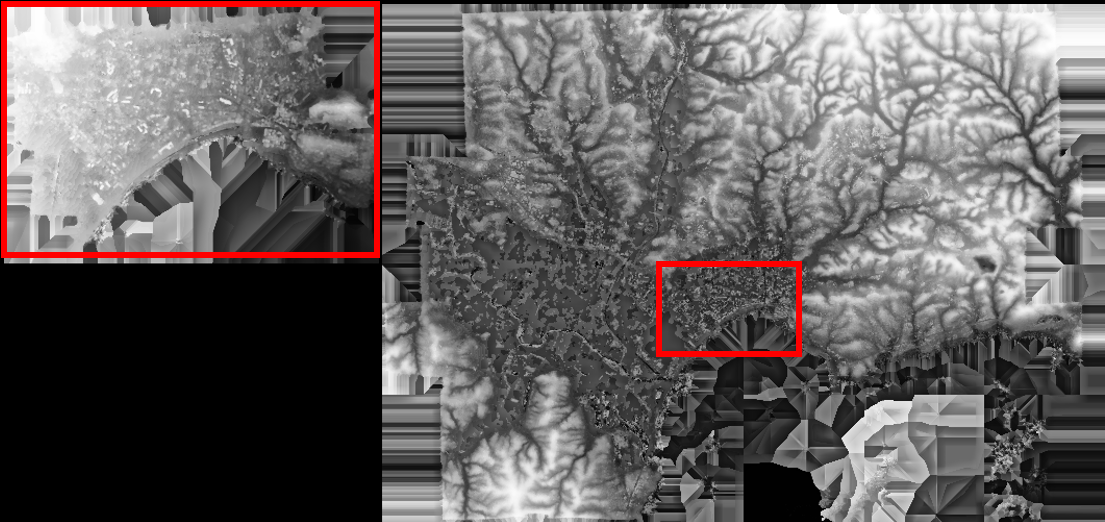
\includegraphics[width=7.5cm]{images/Chapitre3/MEC-Malt_Tapas_1970_MEC-Malt_2014.png}
			\end{minipage}%
		}
		\subfigure[Number of recovered matches]{
			\begin{minipage}[t]{0.48\linewidth}
				\centering
				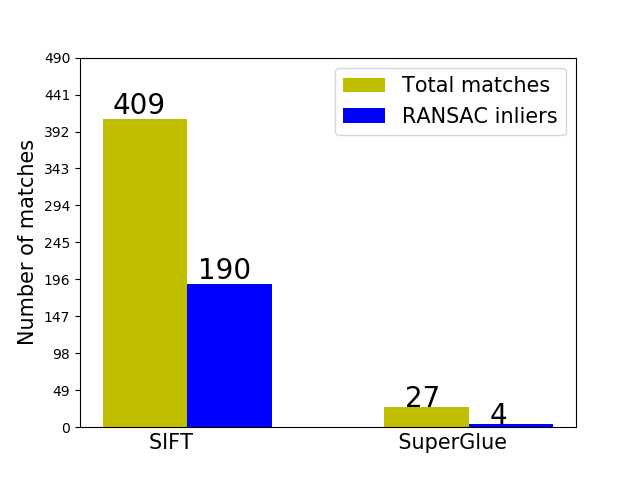
\includegraphics[width=4.8cm]{images/appendix2/PlotCurves_TileTest-MEC-Malt_Tapas_1970_MEC-Malt_2014.png}
			\end{minipage}%
		}
		\subfigure[$SuperGlue_{ours}^{RANSAC Inliers}$]{
			\begin{minipage}[t]{0.48\linewidth}
				\centering
				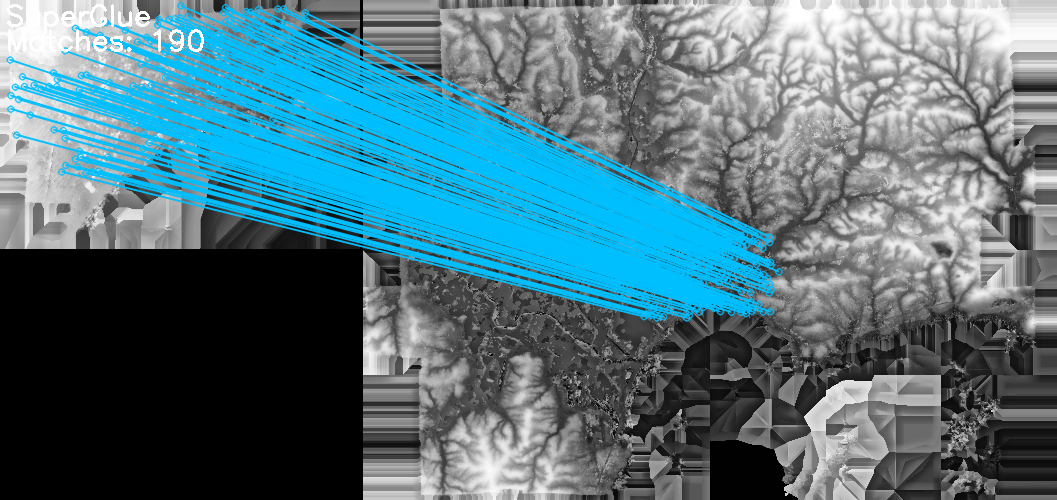
\includegraphics[width=6cm]{images/Chapitre3/Homol-SubPatch_R270-2DRANSAC_MEC-Malt_Tapas_1970_MEC-Malt_2014.png}
			\end{minipage}%
		}
		\subfigure[$SuperGlue_{orig}^{TotalMatches}$]{
			\begin{minipage}[t]{0.48\linewidth}
				\centering
				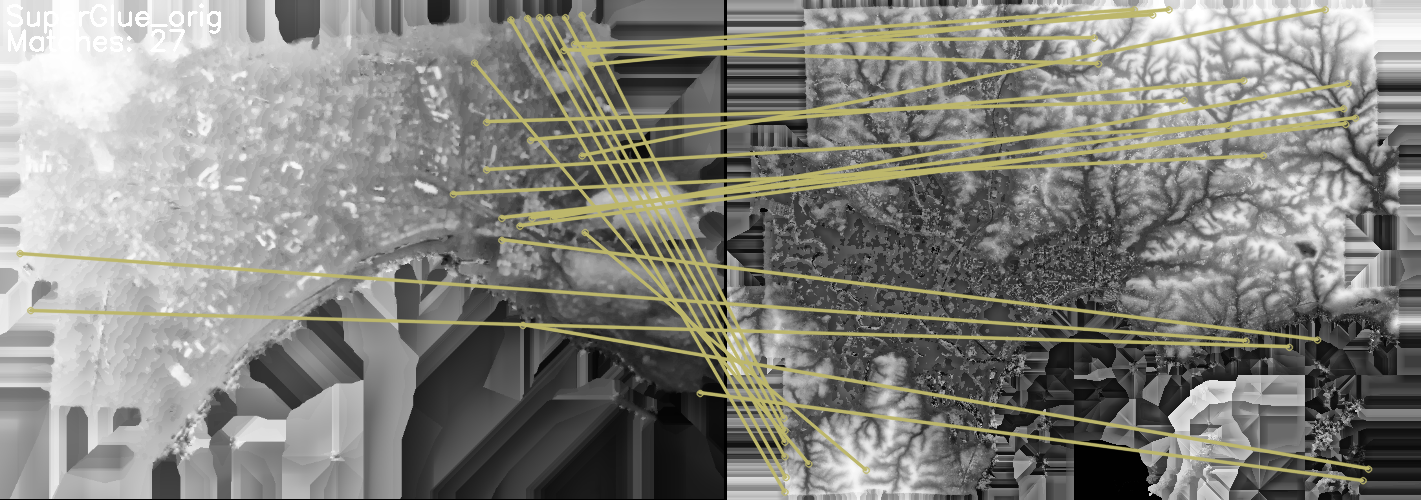
\includegraphics[width=6cm]{images/appendix2/Homol-SuperGlue_MEC-Malt_Tapas_1970_MEC-Malt_2014.png}
			\end{minipage}%
		}
		\caption{Comparison between $SuperGlue_{tiling}$ and $SuperGlue_{orig}$ on DSMs from Fr{\'e}jus 1970 and 2014 individually. (a) DSMs to be matched, with red rectangles indicating the common zone. (b) Numbers of total matches, GT inliers and RANSAC inliers of $SuperGlue_{tiling}$ and $SuperGlue_{orig}$. (c) Visualization of RANSAC inliers based on $SuperGlue_{tiling}$. (d)Visualization of total matches based on $SuperGlue_{orig}$.}
		\label{MatchDSM}
	\end{center}
\end{figure*} 


%And I cite myself to show by bibtex style file (two authors)~\cite{Commowick_MICCAI_2007}.
%This for other bibtex stye file : only one author~\cite{Oakes_RStat_1999} and many authors~\cite{Guimond_CVIU_2000}.
